%%%%%%%%%%%%%%%%%%%%%%%%%%%%%%%%%%%%%
%応用数学 運動座標における運動方程式のメモ
%@maruuusa83
%
%2014.2.5
%%%%%%%%%%%%%%%%%%%%%%%%%%%%%%%%%%%%%

\documentclass[twocolumn,a4j,10pt]{jarticle}
%\documentclass[a4j,10pt]{jarticle}

\usepackage{amsmath,amssymb}
\newtheorem{thm}{定理}

\makeatletter

%パッケージ
\usepackage{bm}
\usepackage[dvipdfmx]{graphicx}
\usepackage{float}

%ヘッダ定義
\usepackage{fancyhdr}
\pagestyle{fancy}
\rhead{applied mathematics}
\cfoot{\thepage}


%文字サイズ定義
\def\section{\@startsection {section}{1}{\z@}{3.5ex plus 1ex minus 2ex}{2.3 ex plus .2ex}{\fontsize{10pt}{0pt}\bf}}
\def\subsection{\@startsection {subsection}{1}{\z@}{3.5ex plus 1ex minus 
2ex}{2.3ex plus .2ex}{\fontsize{10pt}{0pt}\bf}}

%式番号に節番号を含める
\renewcommand{\theequation}{%
\thesection.\arabic{equation}}
\@addtoreset{equation}{section}

%表紙
%
\renewcommand{\maketitle}{\begin{titlepage}%
    \let\footnotesize\small
    \let\footnoterule\relax
    \parindent \z@
    \reset@font
    \null\vfil
    \hrule height 4pt
    \vskip 10\p@
      \LARGE 
      \strut \@title \par
    \begin{flushright}
      \vskip 30\p@
      \strut \@author
    \end{flushright}
    \vskip 5\p@
    \hrule height 4pt
    \vfil
    \begin{flushright}
        {\small \@date}%
    \end{flushright}
  \end{titlepage}%
  \setcounter{footnote}{0}%
}
\makeatother


%ドキュメントの開始%%%%%%%%%%%%%%%%%%%
\begin{document}

%表紙%%%%%%%%%%%%%%%%%%%
\author{marusa}
\title{運動座標系における運動方程式のメモ}
\date{Feb, 2014}

\maketitle

%本文%%%%%%%%%%%%%%%%%%%
\section{前提}
ある観測者が、沖縄高専から宇宙上にある物体を観測したいとする。

観測者は、自身の位置を原点に地球の表面上に座標系を設定して、観測対象の位置
\begin{equation}
  \bm{r}(t) = \sum_{n=1}^{3}x_n \bm{e}_n
  \label{relative_coordinate}
\end{equation}
を観測したという。これは、観測者の状態に依存して様々な値をとるから、\textbf{相対的な観測量}である 

これに対して、絶対静止系に静止している神の観測は
\begin{equation}
  \bm{R}(t) = \sum_{m=1}^{3}X_m \bm{i}_m
  \label{absolute_coordinate}
\end{equation}
である。

地球の中心点の位置を、絶対座標からの位置ベクトルで$\bm{a}$と表し、地球の中心点からの観測者への位置ベクトルを$\bm{b}$と表す。

\begin{figure}[H]
  \centering
 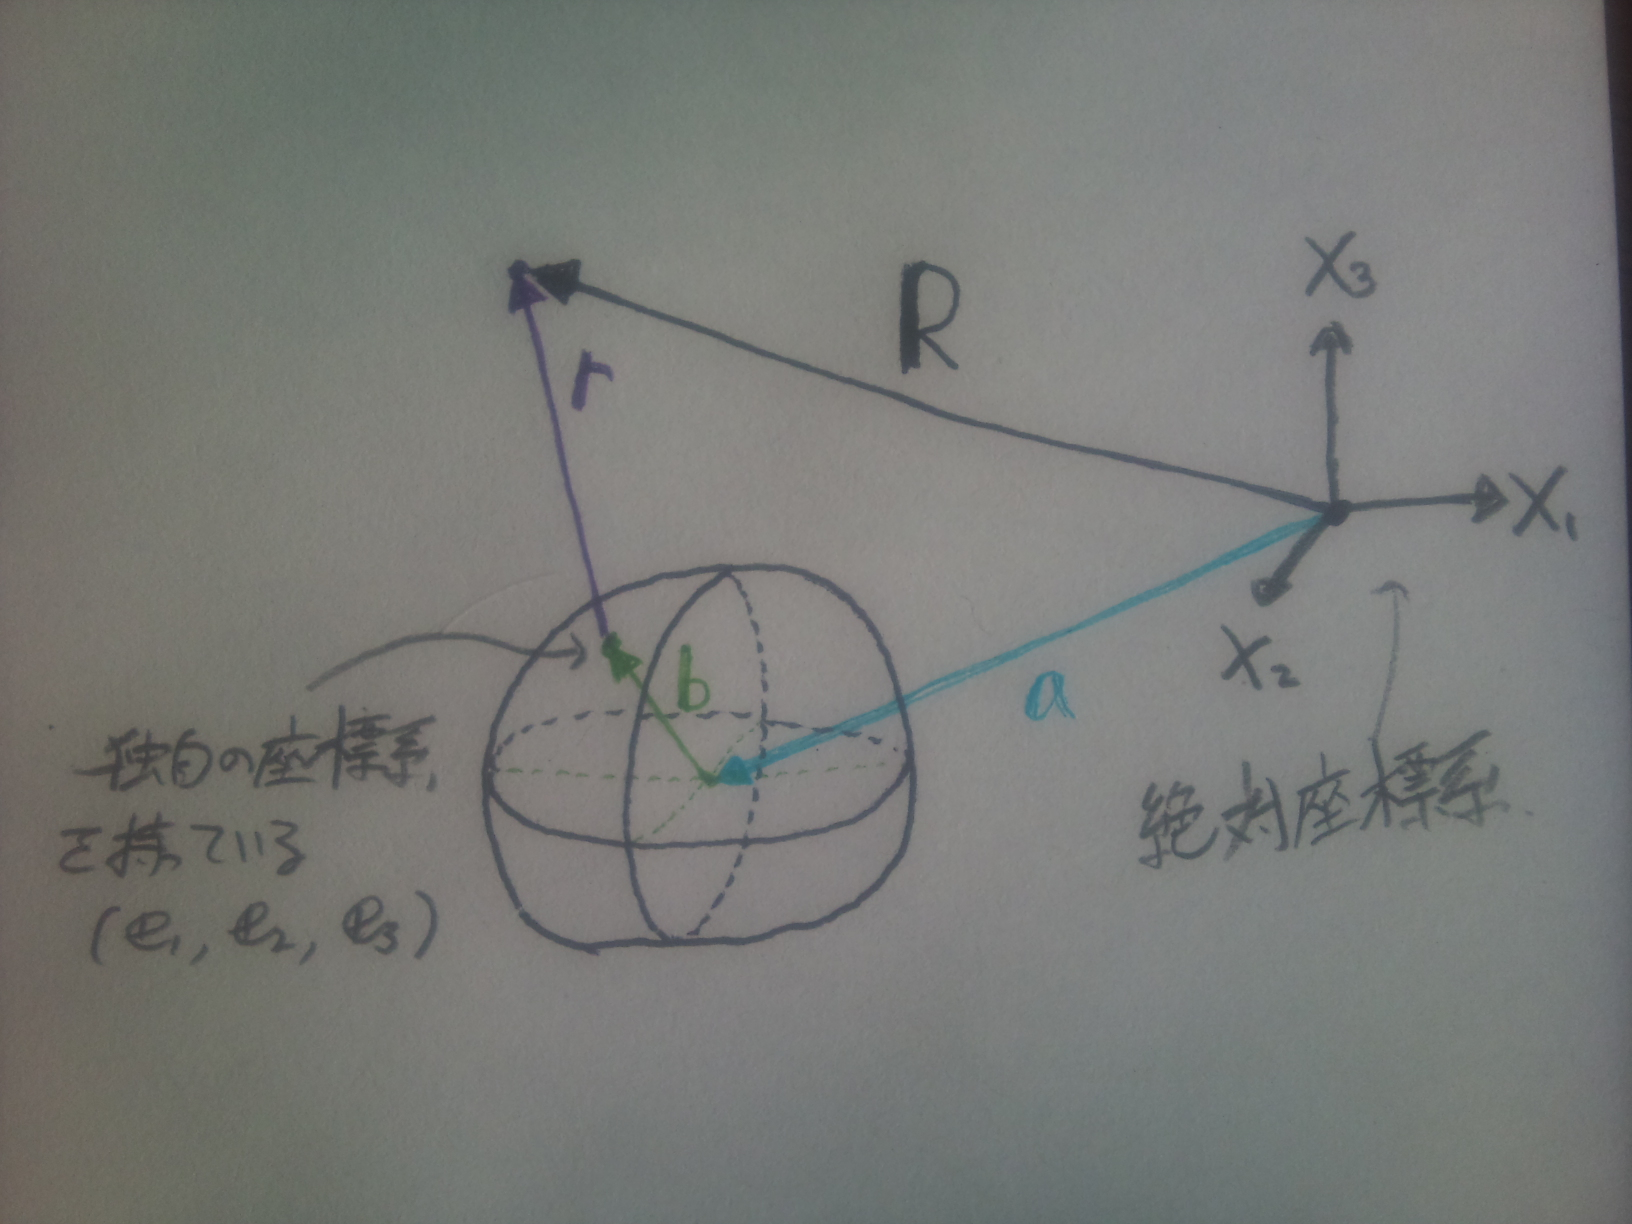
\includegraphics[width=5cm]{./pic/system.jpg}
 \caption{空間の関係図}
 \newline
\end{figure}


\section{目標}
宇宙に存在している物体の絶対座標系における速度を求めることが目標である。

ニュートンは、$\bm{F}$=m$\bm{a}$は絶対静止系(またはそれに同等な慣性座標系)において成り立つとした。すなわち、この場合においての\textbf{観測者は運動座標系を持っている}ので正しい運動方程式が得られない。そのため、相対座標$\bm{r}$を用いて観測対象の正しい運動方程式を定める。

そのため先ず我々は、宇宙に存在している物体の絶対座標系における速度を求める必要がある。\newline


\section{速度を求めることについての考察}
$\bm{R}$と$\bm{r}$の関係は次のように書くことができる。
\begin{equation}
  \bm{R}(t) = \bm{a} + \bm{b}(t) + \bm{r}(t)
  \label{relation_between_R_r}
\end{equation}
ここで、宇宙に存在する物体の速度は、$\bm{R}$を微分することで得ることができる。とはいえ我々は$\bm{R}$は知らない。しかし、$\bm{r}$ならば知っている。
\begin{eqnarray}
  \frac{\mathrm{d}}{\mathrm{d} t} \bm{R} &=& \frac{\mathrm{d}}{\mathrm{d} t} \left\{ \bm{a} + \bm{b}(t) + \bm{r}(t) \right\} \nonumber \\
 &=& \frac{\mathrm{d}}{\mathrm{d} t} \left\{ \bm{a} + \bm{b}(t) + \sum_{n=1}^{3} x_n (t) \bm{e}_n \right\} \nonumber \\
  &=& \bf{v} \nonumber
\end{eqnarray}
地球の位置$\bm{a}$が絶対座標系において不変だとすると、式を整理して
\begin{eqnarray}
  \frac{\mathrm{d}}{\mathrm{d} t} \bm{R} &=& \frac{\mathrm{d} \bm{b}}{\mathrm{d} t} + \frac{\mathrm{d} \bm{r}}{\mathrm{d} t} \nonumber \\
  &=& \frac{\mathrm{d}}{\mathrm{d} t} \bm{b} + \sum_{n=1}^{3} \frac{\mathrm{d}}{\mathrm{d} t}x_n \bm{e}_n
  \label{diff_of_R}
\end{eqnarray}
を得ることができる。(ただし、これが$t$の関数であることを忘れてはいけない。)\newline


\section{観測者の座標系の運動について考える}
宇宙上の物体を観測している観測者は沖縄高専にいるので、\textbf{本人は静止しているつもりでも、絶対座標系においては地球の自転によって運動している。}だから、観測者の座標系が運動していることも検討しなければならない。\newline

自転する地球上に存在する人間が作る座標系であるから、当然この座標系の基底ベクトル$\bm{e}_1,\bm{e}_2,\bm{e}_3$も時間とともにその向きが変化する。

この基底ベクトルの時間微分は、係数を、基底aに対する基底bの貢献度:$\Omega_{ab}$と書くことにしてまとめると、次のようになる。
\begin{equation}
  \left\{ \begin{array}{rl}
\frac{\mathrm{d} }{\mathrm{d} t} \bm{e}_1 = \Omega_{11} \bm{e}_1 + \Omega_{12} \bm{e}_2 + \Omega_{13} \bm{e}_3 \\
\frac{\mathrm{d} }{\mathrm{d} t} \bm{e}_2 = \Omega_{21} \bm{e}_1 + \Omega_{22} \bm{e}_2 + \Omega_{23} \bm{e}_3 \\
\frac{\mathrm{d} }{\mathrm{d} t} \bm{e}_3 = \Omega_{31} \bm{e}_1 + \Omega_{32} \bm{e}_2 + \Omega_{33} \bm{e}_3
  \label{speed_of_observer}
  \end{array} \right.
\end{equation}\newline

ところで、\textbf{円周上を運動する点の位置ベクトルを$\bm{r}$と書くとき、$\bm{r}$の速度ベクトル$\frac{\mathrm{d}\bm{r}}{\mathrm{d}t}$は$\bm{r}$に垂直}であるから、
\begin{equation}
  \frac{\mathrm{d} \bm{e}_1}{\mathrm{d} t} = (係数)\bm{e}_2 + (係数)\bm{e}_3 \nonumber
\end{equation}

と表すことができる。すなわち、あるベクトルの微分は自ベクトルに垂直であるので、自ベクトル方向の成分は持たない。このことから、不要な成分を削除した次の式を得る。

\begin{equation}
  \left\{ \begin{array}{rl}
\frac{\mathrm{d} }{\mathrm{d} t} \bm{e}_1 = \Omega_{12} \bm{e}_2 + \Omega_{13} \bm{e}_3 \\
\frac{\mathrm{d} }{\mathrm{d} t} \bm{e}_2 = \Omega_{23} \bm{e}_3 + \Omega_{21} \bm{e}_1 \\
\frac{\mathrm{d} }{\mathrm{d} t} \bm{e}_3 = \Omega_{31} \bm{e}_1 + \Omega_{32} \bm{e}_2
  \label{speed_of_observer}
  \end{array} \right.
\end{equation}\newline

もう少しこの式を整理しよう。基底ベクトルは直交するので、その内積の値は0である。これを時間$t$で微分すると、
\begin{equation}
  \frac{\mathrm{d} \bm{e}_1}{\mathrm{d} t} \bm{e}_2 + \bm{e}_1 \frac{\mathrm{d} \bm{e}_2}{\mathrm{d} t} = 0 \nonumber
\end{equation}
を得る。

さらに、式(\ref{speed_of_observer})のそれぞれの式において次のように左辺の項が1つ消えるように基底ベクトルの内積をとると、次のような結果が得られる。
\begin{eqnarray}
  \frac{\mathrm{d} \bm{e}_1}{\mathrm{d} t} \cdot \bm{e}_2 &=& \Omega_{12} \bm{e}_2 \cdot \bm{e}_2 + \Omega_{13} \bm{e}_3 \cdot \bm{e}_2 \nonumber \\
  &=& \Omega_{12} \nonumber
\end{eqnarray}
この内積は、$\bm{e}_1$方向の速度ベクトル$\frac{\mathrm{d} \bm{e}_1}{\mathrm{d} t}$の$\bm{e}_2$に対する射影の大きさが$\Omega_{12}$であることを示している。\newline

この2つの性質を用いると、それぞれの貢献度は次の関係を持つことがわかる。
\begin{eqnarray}
  \Omega_{12} + \Omega_{21} = 0 \nonumber \\
  \Omega_{23} + \Omega_{32} = 0 \nonumber \\
  \Omega_{31} + \Omega_{13} = 0 \nonumber
\end{eqnarray}
このことから、式(\ref{speed_of_observer})の貢献度を3種類にまとめて次のように書き直すことができる。

\begin{equation}
  \left\{ \begin{array}{rl}
\frac{\mathrm{d} }{\mathrm{d} t} \bm{e}_1 = \Omega_{12} \bm{e}_2 - \Omega_{31} \bm{e}_3 \\
\frac{\mathrm{d} }{\mathrm{d} t} \bm{e}_2 = \Omega_{23} \bm{e}_3 - \Omega_{12} \bm{e}_1 \\
\frac{\mathrm{d} }{\mathrm{d} t} \bm{e}_3 = \Omega_{31} \bm{e}_1 - \Omega_{23} \bm{e}_2
  \label{speed_of_observer_2}
  \end{array} \right.
\end{equation}

この式は次の章の最後に用いる。


\section{$\bf{r}$の一階微分の幾何学的意味}
式(\ref{diff_of_R})で現れた、$\bm{r}$の変化率を表す式
\begin{equation}
  \frac{\mathrm{d} \bm{r}}{\mathrm{d} t} = \sum_{n=1}^{3} \frac{\mathrm{d}}{\mathrm{d} t}x_n \bm{e}_n
  \label{deff_of_small_r}
\end{equation}
について考えていこう。

先ずはこの式が幾何学的に何を意味しているのか考える。
\begin{eqnarray}
  \frac{\mathrm{d} \bm{r}}{\mathrm{d} t} &=& \sum_{n=1}^{3} \frac{\mathrm{d}}{\mathrm{d} t} x_n \bm{e}_n \nonumber \\
  &=& \frac{\mathrm{d}}{\mathrm{d} t} (x_1 \bm{e}_1)
      + \frac{\mathrm{d}}{\mathrm{d} t} (x_2 \bm{e}_2)
      + \frac{\mathrm{d}}{\mathrm{d} t} (x_3 \bm{e}_3) \nonumber \\
  &=& \frac{\mathrm{d}}{\mathrm{d} t} x_1 \cdot \bm{e}_1 + x_1 \frac{\mathrm{d}}{\mathrm{d} t} \bm{e}_1 \nonumber \\
  &+& \frac{\mathrm{d}}{\mathrm{d} t} x_2 \cdot \bm{e}_2 + x_2 \frac{\mathrm{d}}{\mathrm{d} t} \bm{e}_2 \nonumber \\
  &+& \frac{\mathrm{d}}{\mathrm{d} t} x_3 \cdot \bm{e}_3 + x_3 \frac{\mathrm{d}}{\mathrm{d} t} \bm{e}_3 \nonumber
\end{eqnarray}
この式を、観測値に関する微分の項と基底ベクトルに関する微分の項に分けて整理すると、次式のようにまとめられる。
\begin{eqnarray}
  \frac{\mathrm{d} \bm{r}}{\mathrm{d} t} &=& \left\{ \frac{\mathrm{d}}{\mathrm{d} t} x_1 \cdot \bm{e}_1 + \frac{\mathrm{d}}{\mathrm{d} t} x_2 \cdot \bm{e}_2 + \frac{\mathrm{d}}{\mathrm{d} t}  x_3 \cdot \bm{e}_3 \right\} \nonumber \\
  &+& \left\{ x_1 \frac{\mathrm{d}}{\mathrm{d} t} \bm{e}_1 + x_2 \frac{\mathrm{d}}{\mathrm{d} t} \bm{e}_2 + x_3 \frac{\mathrm{d}}{\mathrm{d} t} \bm{e}_3 \right\}
  \label{deff_of_R_2}
\end{eqnarray}

式(\ref{deff_of_R_2})の初項は、観測した$\bm{r}$の成分ごとの微分なので、\textbf{観測者の座標系からみた宇宙に存在する物体の速度ベクトル}である。また、第二項は座標系自身の変化率を表しているので、\textbf{観測者の座標系自身の速度ベクトル}である。\newline

\section{観測者座標系の速度を求める}
さて、この式(\ref{deff_of_R_2})の第二項に、4章で求めた式(\ref{speed_of_observer_2})を代入して、基底ベクトルごとに整理してみる。
\begin{eqnarray}
  & & x_1 \frac{\mathrm{d}}{\mathrm{d} t} \bm{e}_1 + x_2 \frac{\mathrm{d}}{\mathrm{d} t} \bm{e}_2 + x_3 \frac{\mathrm{d}}{\mathrm{d} t} \bm{e}_3 \nonumber \\
  &=& x_1 \left( \Omega_{12} \bm{e}_2 - \Omega_{31} \bm{e}_3 \right) \nonumber \\
  &+& x_2 \left( \Omega_{23} \bm{e}_3 - \Omega_{12} \bm{e}_1 \right) \nonumber \\
  &+& x_3 \left( \Omega_{31} \bm{e}_1 - \Omega_{23} \bm{e}_2 \right) \nonumber \\
  &=& \left( x_3 \Omega_{31} - x_2 \Omega_{12} \right) \bm{e}_1 \nonumber \\
  &+& \left( x_1 \Omega_{12} - x_3 \Omega_{23} \right) \bm{e}_2 \nonumber \\
  &+& \left( x_2 \Omega_{23} - x_1 \Omega_{31} \right) \bm{e}_3
  \label{deff_of_R_3}
\end{eqnarray}

ここで、$\Omega_{12},\Omega_{23},\Omega_{31}$を改めて$\Omega_{3},\Omega_{1},\Omega_{2}$と書くことにして、行列形式表示にすると、見やすくまとまる。

\begin{eqnarray}
  & & x_1 \frac{\mathrm{d}}{\mathrm{d} t} \bm{e}_1 + x_2 \frac{\mathrm{d}}{\mathrm{d} t} \bm{e}_2 + x_3 \frac{\mathrm{d}}{\mathrm{d} t} \bm{e}_3 \nonumber \\
  &=& \left( \begin{array}{c}
    \Omega_1 \\
    \Omega_2 \\
    \Omega_3
  \end{array} \right)
  \times 
  \left( \begin{array}{c}
    x_1 \\
    x_2 \\
    x_3
  \end{array} \right)
\end{eqnarray}

式中の、貢献度$\Omega_n$を成分に持つベクトルを$\bm{\Omega}$と名付ければ、次のように非常に美しい形にまとめることができる。
\begin{equation}
  x_1 \frac{\mathrm{d}}{\mathrm{d} t} \bm{e}_1 + x_2 \frac{\mathrm{d}}{\mathrm{d} t} \bm{e}_2 + x_3 \frac{\mathrm{d}}{\mathrm{d} t} \bm{e}_3 = \bm{\Omega} \times \bm{r}
  \label{angular_speed}
\end{equation}\newline


\section{$\bm{r}$の一階微分}
改めて式(\ref{deff_of_R_2})を整理しよう。
\begin{eqnarray}
  \frac{\mathrm{d} \bm{r}}{\mathrm{d} t} &=& \left\{ \frac{\mathrm{d}}{\mathrm{d} t} x_1 \cdot \bm{e}_1 + \frac{\mathrm{d}}{\mathrm{d} t} x_2 \cdot \bm{e}_2 + \frac{\mathrm{d}}{\mathrm{d} t}  x_3 \cdot \bm{e}_3 \right\} \nonumber \\
  &+& \left\{ x_1 \frac{\mathrm{d}}{\mathrm{d} t} \bm{e}_1 + x_2 \frac{\mathrm{d}}{\mathrm{d} t} \bm{e}_2 + x_3 \frac{\mathrm{d}}{\mathrm{d} t} \bm{e}_3 \right\} \nonumber \\
  &=& \left( \begin{array}{c}
    \frac{\mathrm{d}}{\mathrm{d} t} x_1 \\
    \frac{\mathrm{d}}{\mathrm{d} t} x_2 \\
    \frac{\mathrm{d}}{\mathrm{d} t} x_3 \\
  \end{array} \right)
  + \bm{\Omega} \times \bm{r} \nonumber \\
  &=& \bm{v}_r + \bm{\Omega} \times \bm{r} 
  \label{deff_of_R_3}
\end{eqnarray}

観測者からみた宇宙の物体の位置の微分を$\bm{v}_r$と置き換えた。幾何学的考察の章でも述べたが、$\bm{v}_r$は観測者からみた宇宙上の物体の速度ベクトルである。\newline


\section{$\bm{r}$の一階微分に関するまとめ}
ここで、もう一度目指す先を思い出そう。宇宙上に存在する物体の絶対座標系における速度を求めたいのであった。そのためには$\bm{R}$を微分する必要があったが我々に$\bm{R}$を知る術はなかった。であるので、式(\ref{diff_of_R})を用いて絶対静止系における速度を求める試みを行っている。

\begin{equation}
  \frac{\mathrm{d} \bm{R}}{\mathrm{d} t} = \frac{\mathrm{d} \bm{b}}{\mathrm{d} t} + \frac{\mathrm{d} \bm{r}}{\mathrm{d} t} \nonumber
\end{equation}

そして我々は$\bm{r}$の一階微分の値を手に入れることができた。すなわち、
\begin{equation}
  \frac{\mathrm{d} \bm{R}}{\mathrm{d} t} = \frac{\mathrm{d} \bm{b}}{\mathrm{d} t} + \bm{v}_r + \bm{\Omega} \times \bm{r}
 \label{diff_of_R_5}
\end{equation}
を手に入れた。次は、$\bm{b}$の微分を求めることにしよう。\newline


\section{$\bm{b}$を求める}
観測者が地球の表面上で常に静止しているのであれば、$\bm{b}$は地球の自転のための変化であると考えられる。

\begin{figure}[H]
  \centering
 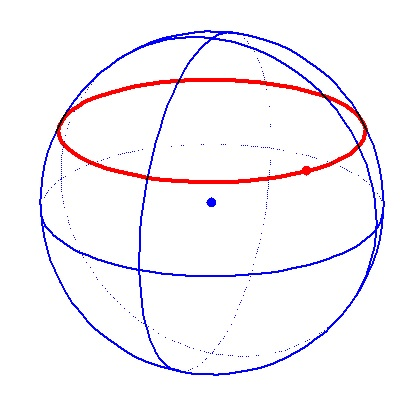
\includegraphics[width=5cm]{./pic/rot.jpg}
 \caption{地球の自転による観測者の軌道}
 \newline
\end{figure}

ところでこれは、第6章で求めた観測者自身の速度であるので、式(\ref{deff_of_R_3})をそのまま使うことができる。
すなわち、絶対座標系からみた地球の自転による観測者の運動は
\begin{equation}
  \frac{\mathrm{d} \bm{b}}{\mathrm{d} t} = \bm{\Omega} \times \bm{b} 
  \label{diff_of_b}
\end{equation}
と表すことができる。\newline


\section{$\bm{R}$の一階微分を得る}
$\bm{b}$の一階微分が得られた。式(\ref{diff_of_R_5})に、得られた式(\ref{diff_of_b})を代入すれば、$\bm{R}$の一階微分を得る。

\begin{eqnarray}
  \frac{\mathrm{d} \bm{R}}{\mathrm{d} t} &=& \bm{\Omega} \times \bm{b} + \bm{v}_r + \bm{\Omega} \times \bm{r} \nonumber \\
  &=& \bm{v}_r + \Omega \times \left\{ \bm{b} + \bm{r} \right\}
 \label{diff_of_R_6}
\end{eqnarray}

これでRの一階微分、すなわち絶対座標系における宇宙に存在する物体の速度を求めることができた。

\end{document}


























